\documentclass[12pt]{article}
\usepackage[12pt]{moresize}
\usepackage[margin=1in]{geometry}

\usepackage{amsmath}
\usepackage{amssymb}

\usepackage{graphicx}
\usepackage{subcaption}

\usepackage{multirow} %Combining rows in tables
\usepackage{diagbox}  %Table box split in twain

\usepackage{algorithm}
\usepackage{algpseudocode}
\usepackage{alltt}

\usepackage{multicol}

\usepackage{amssymb} %\checkmark symbol

%\usepackage{hyperref}
%\usepackage[latin1]{inputenc}
%\usepackage{listings}
%\usepackage{scrextend}
%\usepackage{changepage} %Adjustwidth

 

\title{ComS 472\\Homework 2}
\author{Sean Gordon}
\date{Sep 25, 2020}

\begin{document}
\maketitle


\centerline{- 4.1 - }
\ \\
\noindent 1) Hill climb search\\
2) Breadth first search, adding one layer of nodes at a time\\
3) First Choice Hill climb search, as T=0 effectively removes temperature from the algorithm\\
4) Random walk, as temperature would cause every successor to have equal probability\\
5) Random walk, as the only chance for movement would be mutation


\noindent \hrulefill \\


\centerline{- 4.7 - }
\ \\
\noindent As the initial belief state contains all possible states, and we know the true cost for each state, a good heuristic for an individual belief states is the maximum of the costs of the states it contains. As you can never know which specific state in a belief state you are in, you must assume the worst case (the largest cost state). Because any solution for this largest cost state would also solve the other states in the belief state, this heuristic is admissible.


\noindent \hrulefill \\



\centerline{- 4.8 - }
\ \\
\noindent 1. A solution for b would pass through the subsets of b, and thus would be a solution from those subsets. Because the solution doesn't necessarily pass through the superstates of b, it is not a solution for the supersets.\\

\noindent 2. Graph search can be optimized for this problem by keeping a list of visited nodes. If the current node has already been visited, we can skip it and its children. This will avoid loops that needlessly increase the cost.\\



\noindent \hrulefill \\\pagebreak


\centerline{- 4.10 - }
\begin{figure}[htbp]
\centerline{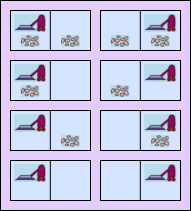
\includegraphics{Pics/ComS472_410.png}}
\caption{Belief states recheable from initial 8 belief states.}
\label{Belief states recheable from initial 8 belief states.}
\end{figure}

The problem is unsolvable because of the chance of depositing dirt when cleaning an empty square. Because there are no sensors, the agent can't tell if a square is initially clean or not and may end up depositing dirt when sucking, so the possible belief states can never be reduced.


\noindent \hrulefill \\\pagebreak


\centerline{- 5.8 - }
\begin{figure}[htbp]
\centerline{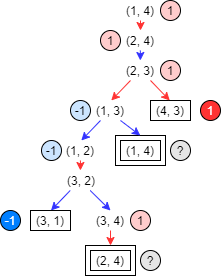
\includegraphics{Pics/ComS472_58ptB.png}}
\caption{Line Game tree.}
\label{Line Game tree.}
\end{figure}

Because the ? values corresponded to loop positions that were always higher in the tree, they would be considered anyway as the algorithm propagates upward. Therefore, I just propagated the ? and ignored it when faced with a choice.\\

Minimax operates using DFS, and would therefore be stuck in an infinite loop upon reaching a loop position. This can be avoided by keeping a record of visited states, and skipping any that have been visited already.\\

If both players are playing optimally, the game is decided in the center of the box, with the win going to the first player to jump over the other, putting them 1 square closer to goal than the opposition. If n is even, A reaches the center line first and is poised to jump over B. If it is odd, A moves past the center line first, and B is poised to jump over A.\\


\noindent \hrulefill \\\pagebreak



\centerline{- 5.9 - }
\ \\
\centerline{There are 255168 unique games possible}
\begin{figure}[htbp]
\centerline{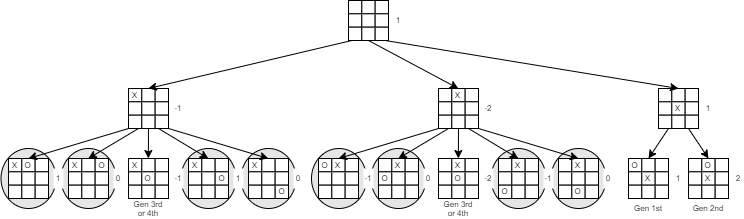
\includegraphics[scale=.75]{Pics/ComS472_59.png}}
\caption{Tic-Tac-Toe tree.}
\label{Tic-Tac-Toe tree.}
\end{figure}




\noindent \hrulefill \\



\centerline{- 5.14 - }
\ \\
\noindent 1) $n_1 = min( max(n_3, n_{31}, ..., n_{3j_3}), n_{21}, ..., n_{2b_2}) $\\
\noindent 2) $n_1 = min(l_2,  max(l_3, n_3, r_3), r_2) $\\
\noindent 3) $n_1 = min(l_2,  max(min(min(l_3, l_{31}, ..., l_{3j}),  n_3, r_3), r_2) $\\
$n_j$ must not exceed the upper bound placed on it by all nodes to its left ($l_2, l_4, ..., l_i$), or it will not be selected higher up in the tree. I have no idea how to reformat this expression to show that without it being an absolute mess... \\
\noindent 4) I still don't know how to reformat that expression, but the lower bound for this one is $max(l_3, l_5, ..., l_j)$.\\


\noindent \hrulefill \\\pagebreak



\centerline{- Extra - }
\ \\
\centerline{The final value for root is 14.}
\begin{figure}[htbp]
\centerline{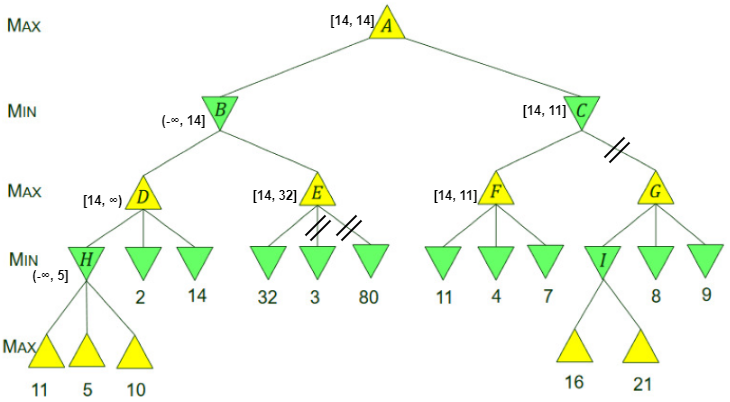
\includegraphics[scale=.75]{Pics/ComS472_Extra.png}}
\caption{Alpha-Beta tree.}
\label{Alpha-Beta tree.}
\end{figure}


\end{document}

















